\section{Probability Theory}
\label{sec:probability-theory}
In general, probability reflects the level of confidence that an event will happen. If, for example,
the weather forecast says, that it will rain with a probability of $0.9$ (or $90\%$), it is
advisable to bring weather-proof clothes when going outside. In order to migrate from this
day-to-day life view on probability to a more formal representation, it is necessary to define what
an event is that a probability is assigned to.

First we define a \emph{sample space} $\Omega$ of possible outcomes of a random experiment or
observation~\citep[17]{billingsley_95_probability}. Furthermore,
the non-empty set $\mathcal{S}$ of \emph{measurable events} or \emph{$\sigma$-algebra} contains those outcomes $\mathcal{S} \ni
\alpha \subseteq \Omega$ which we intend to assign probabilities to.
\begin{mydef}[{\citealp[1]{durrett_10_probability}}]
    \label{def:sigma-algebra}
    A \emph{$\sigma$-algebra} $\mathcal{S}$ is a non-empty collection of subsets $\alpha$ of
    $\Omega$ that satisfy
    \begin{enumerate}
          \item $\emptyset \in \mathcal{S} \wedge \Omega \in \mathcal{S}$. \label{itm:sample-space-one}
          \item Closure under union: $\alpha, \beta \in \mathcal{S} \Rightarrow \alpha \cup \beta \in
        \mathcal{S}$ \label{itm:sample-space-two}
          \item Closure under complementation: $\alpha \in \mathcal{S} \Rightarrow \Omega \setminus
        \alpha \in \mathcal{S}$ \label{itm:sample-space-three}
    \end{enumerate}
\end{mydef}
% These constrictions lay the foundations for the definition of a probability distribution.
The pair $(\Omega, \mathcal{S})$ is called a \emph{measurable space}. Then, a \emph{probability
    distribution} can be defined on a measurable space.

\begin{mydef}[{\citealp[17]{koller_09_probabilistic}}]
    \label{def:probability}
    A \emph{probability distribution} $P$ over $(\Omega, \mathcal{S})$
    \begin{align}
        \label{eq:probability-mapping}
        P: \mathcal{S} &\to [0,1] \subset \mathbb{R} \\ \nonumber
        \alpha &\mapsto P(\alpha)
    \end{align}
    maps the outcome $\alpha \in \mathcal{S}$ of a random experiment to a real number $P(\alpha)$ in
    the interval $[0,1]$. In addition, it fulfills the \emph{Kolmogorov axioms}:
    \begin{enumerate}
          \item $P(\alpha) \ge 0 \; \forall \alpha \in \mathcal{S}$
          \item $P(\Omega) = 1$ \label{itm:probability-trivial}
          \item $\alpha, \beta \in \mathcal{S} \wedge \alpha \cap \beta = \emptyset \Rightarrow
        P(\alpha \cup \beta) = P(\alpha) + P(\beta)$ \label{itm:probability-union}
    \end{enumerate}
\end{mydef}
Note that the second and third of the Kolmogorov axioms impose normalization of the probability
distribution and assign zero probability to the empty event:
\begin{align}
    \label{eq:probability-no-empty-event}
    &&P(\Omega) = P(\Omega \cup \emptyset) = P(\Omega) + P(\emptyset) \\
    &\Leftrightarrow &P(\Omega) - P(\Omega) = P(\Omega) - P(\Omega) + P(\emptyset) \\
    &\Leftrightarrow &P(\emptyset) = 0
\end{align}
The Bayesian interpretation sees probability as a degree of confidence in between the two extrema
$P(\alpha)=1$ and $P(\alpha)=0$ for event $\alpha \in \mathcal{S}$ as an outcome of a random
experiment. From a frequentist point of view, that is the fraction of outcomes in the limit of
infinite repetitions of the random experiment.

% When the quantity of interest is not the probability of an event $\beta$, but the probability
% of event $\beta$ given the knowledge about event $\alpha$, or -- more formal -- conditioned on event
% $\alpha$, 
\begin{mydef}[{\citealp[18]{koller_09_probabilistic}}]
    \label{def:conditional-probability}
    \emph{The conditional} probability of $\beta$ given $\alpha$
    \begin{align}
        \label{eq:condititonal-probability}
        P(\beta | \alpha) = \frac{P(\alpha \cap \beta)}{P(\alpha)}, \; P(\alpha) \ne 0
    \end{align}
    is the probability that $\beta$ will happen, given knowledge about
    $\alpha$.
\end{mydef}
Notably, $P(\beta | \alpha)$ fulfills all requirements from \cref{def:probability} and therefore is
a probability distribution.

A direct consequence of \cref{eq:condititonal-probability} is \emph{Bayes' theorem}~\citep[15]{bishop_07_pattern}:
\begin{align}
    \label{eq:bayes-theorem}
    P(\alpha|\beta)P(\beta) = P(\beta|\alpha)P(\alpha)
\end{align}
    

% \label{sec:probability-theory}
% \begin{mydef}
%     \label{def:gm-space}
%     The \emph{sample space} $\Omega$ consists of all possible outcomes $\omega$ of a random experiment or
%     observation\citep{billingsley_95_probability}~\citep[17]{billingsley_95_probability}. 
% \end{mydef}

% \citet{billingsley_95_probability}{17}

Hitherto, \cref{def:probability} provides a distribution over the abstract space of events $\alpha
\in \mathcal{S}$ that are sets of possible outcomes ($\alpha \subseteq \Omega$). For the application
on real world problems, it is more intuitive to model distributions over attributes of the outcome
rather than the outcome itself. Then, \emph{random variables} provide the means to inject attributes
of the outcome.

\begin{mydef}[{\citealp[8]{durrett_10_probability}}]
    \label{def:random-var}
    A \emph{random variable} $X$ is a function
    \begin{align}
        \label{eq:random-var}
        X:\Omega &\to \val(X) \\
        \omega &\mapsto X(\omega) = x
    \end{align}
    that assigns a realization $x$ of the random variable $X$ to the outcome of a random
    experiment. Here, $\val(X)$ denotes the range of values that
    $X$ can take, most commonly real or natural numbers or subsets thereof.
\end{mydef}
Throughout this thesis, random variables are denoted by a capital letter with realizations depicted
by the appropriate lower case counterpart.
% Furthermore, all random variables take discrete values,
% \ie $\val(X) \subset \mathbb{N} \cup \{0\}$ and $|val(X)| = m < \infty$, unless stated
% otherwise.
Then, 
\begin{align}
    P(X=x)=P\left(\{\omega \in \Omega : X(\omega) = x\}\right)
\end{align}
is the probability that random variable $X$ takes the value $x$ and
\begin{align}
    \sum_{X} = \sum_{x \in \val(X)}
\end{align}
denotes summation over all possible values of $X$. With the introduced convention that a random
variable and its realization form a pair of corresponding lower case and upper case letters, it is
obvious that $x$ always refers to the realization of random variable $X$. Thus, $P(X=x)$ can be
written as $P(x)$ for brevity, when appropriate. Furthermore, sets of random variables are denoted
by calligraphic letters. In general, it is sensible to form sets of random variables that have the
same range of values or that can be grouped semantically. As a final abbreviation, $P(X=x,Y=y)$ and
$P(x,y)$ are shortcuts for the \emph{joint distribution} over $X$ and $Y$ $P\left((X=x) \cap
    (Y=y)\right)$. More generally, this holds for a joint distribution of any number of random
variables: $P(x_1,\hdots,x_N) = P\left(\bigcap_{i=1}^N(X_i=x_i)\right)$. These notational details
are subsumed in \cref{tab:probability-notation}.

In the following, properties of probability distribution over discrete random variables are
introduced. In a similar fashion and with slight modifications, these properties hold for continuous
random variables as well: Sums are exchanged for integrals and the properties are described in terms
of a \emph{probability density function}, typically denoted by $p(\cdot)$, instead of the
probability distribution. In this context, it is important to note that, formally, a distribution
over a continuous random variable describes the probability that the random variable takes a value
in a specified interval rather than a certain value. In spite of this distinction, the probability
density function is commonly referred to as probability distribution. For discrete variables,
however, the intuitive interpretation of assigning probabilities to the states of a random variable
holds. A more in depth presentation of distributions in general and distributions over continuous
random variables in particular can be found in
\citet{durrett_10_probability,billingsley_95_probability,chung_68_course}.

\begin{table}
    \centering
    \begin{tabular}{ll}
        \toprule
        Notation & Meaning \\ \midrule
        $X$ & random variable \\
        $\val(X)$ & value range of $X$ \\
        $X \in A$ & short for $\val(X)=A$ \\
        $x$ & realization of $X$ \\
        $P\left(\{\omega \in \Omega : X(\omega) = x\}\right)$  & probability of $X$ to take value $x$ \\
        $P(X=x)$ & $P\left(\{\omega \in \Omega : X(\omega) = x\}\right)$ \\
        $P(x)$ & $P(X=x)$ \\
        $\mathcal{X}$ & set of random variables $\{X_i\}_{i=1,\hdots,N}$ \\
        $P\left(\bigcap_{i=1}^N(X_i=x_i)\right)$ & joint distribution over set of
        $N$ random variables \\ 
        $P(x_1,\hdots,x_N)$ & $ P\left(\bigcap_{i=1}^N(X_i=x_i)\right)$ \\
        $\sum_{\mathcal{X}}$ & Summation over all possible states of $\mathcal{X}$ \\
        \bottomrule
    \end{tabular}
    \caption[Probability: Notations]{Notations and abbreviations for random variables and probability distributions.}
    \label{tab:probability-notation}
\end{table}

\begin{mydef}
    \label{def:marginalization}
    Given a set of random variables $\mathcal{X} = \{X_1,\hdots,X_N\}$, a \emph{marginal
        distribution} is a probability distribution on a subset of variables
    $\{\hat{X}_1,\hdots,\hat{X}_M\} = \hat{\mathcal{X}} \subset \mathcal{X}$, such that
    \begin{align}
        \label{eq:marginalization}
        P(\hat{x}_1,\hdots,\hat{x}_M) &= \sum_{X_{i_1}}\cdots\sum_{X_{i_{N-M}}}P(x_1,\hdots,x_N), \\
        \left\{X_{i_k}\right\}_{k=1,\hdots,N-M} &= \mathcal{X} \setminus \mathcal{\hat{X}}.
    \end{align}
\end{mydef}
Here, the set $\left\{X_{i_k}\right\}_{k=1,\hdots,N-M}$ denotes all random variables that are in the
original set of variables $\mathcal{X}$, but not in its subset $\hat{\mathcal{X}}$. These $N-M$
variables are ``marginalized out'' by summation over their $N-M$ value ranges. For the purpose of
explanation, take the distribution $P(x, y)$ over two random variables $X$ and $Y$ as an
example. Marginalizing over $Y$ then results in the distribution
\begin{align}
    \label{eq:probability-marginal-example}
    P(x) = \sum_{y \in \val(Y)}P(x, Y=y).
\end{align}
This example is visualized in \cref{fig:probability-example-marginal} with $\val(X)=\{x \in
\mathbb{N} : x \le 9\}$ and \mbox{$\val(Y)=\{1, 2\}$}. In addition,
\cref{fig:probability-example-conditional} shows a conditional distribution of $P(x,y)$. Note that
for random variables conditional probability
\begin{align}
    \label{eq:random-variable-conditional}
    P(x|y) = \frac{P(x,y)}{P(y)}
\end{align}
is defined analogously to \cref{def:conditional-probability}. Therefore, Bayes' theorem
(\cref{eq:bayes-theorem})
\begin{align}
    \label{eq:bayes-theorem-rv}
    P(x|y)P(y) = P(y|x)P(x)
\end{align}
holds for random variables as well. The different natures of a marginal distribution and a
conditional distribution is visualized in \cref{fig:probability-vis}. Once again, this visualization
stresses that, generally speaking, marginalizing and conditioning are not the same. However, when
equality holds, $X$ and $Y$ are considered marginally independent (\cref{eq:probability-marginal-independence-v2}).
\begin{mydef}[{\citealp[10]{barber_12_bayesian}}]
    \label{def:independence}
    Two variables $X$ and $Y$ are \emph{marginally independent} if their joint probability
    factorizes into the product of their marginals:
    \begin{align}
        \label{eq:probability-marginal-independence}
        P(x,y) = P(x)P(y).
    \end{align}
    Then, $X \independent Y$ denotes marginal independence of $X$ and $Y$. The generalization to
    sets of variables $\mathcal{X}$ and $\mathcal{Y}$ can be formulated likewise:
    \begin{align}
        \label{eq:probability-marginal-independence-sets}
        P(x_1,\hdots x_N, y_1,\hdots, y_M) = P(x_1,\hdots x_N)P(y_1,\hdots, y_M)
    \end{align}
\end{mydef}
The abstract \cref{def:independence} can be interpreted meaningfully in that sense, that knowledge
of $Y$ does not change the probability for $X$. Moreover, combining
\cref{eq:bayes-theorem-rv,eq:probability-marginal-independence} for non-zero distributions $P(x) \ne
0$ and $P(y) \ne 0$, yields
\begin{align}
    \label{eq:probability-marginal-independence-v2}
    P(x|y) = P(x) \;\forall y \Leftrightarrow P(y|x) = P(y) \; \forall x,
\end{align}
a mathematical formulation of this interpretation. In \cref{fig:probability-example-joint}, the
distribution over $X$ is clearly dependent on the choice of $Y$: The distribution over $X$ in the
bottom row differs from the distribution over $X$ in the top row. Thus, $X$ and $Y$ are not marginally
independent, $X \not \independent Y$.

More often than being marginally independent, sets of variables are independent conditioned on an
additional set of variables.
\begin{mydef}[{\citealp[7]{barber_12_bayesian}}]
    \label{def:probability-conditional-independence}
    Let $\mathcal{X}$, $\mathcal{Y}$, $\mathcal{Z}$ be sets of random variables. Then $\mathcal{X}$
    and $\mathcal{Y}$ are called \emph{conditionally independent} on $\mathcal{Z}$ under the
    distribution P, if P satisfies
    \begin{align}
        \label{eq:conditional-independence}
        P(\mathcal{X}, \mathcal{Y}|\mathcal{Z}) =
        P(\mathcal{X}|\mathcal{Z})P(\mathcal{Y}|\mathcal{Z}).
    \end{align}
    Conditional independence $\mathcal{X} \independent \mathcal{Y} \;|\; \mathcal{Z}$ is denoted in the
    same manner as marginal dependence.
\end{mydef}
Note that the formulation \cref{eq:conditional-independence} allows for formulating marginal
independency in terms of conditional independency: Two sets of variables $\mathcal{X}$ and
$\mathcal{Y}$ are marginally independent if they are independent conditioned on the empty set, or
formally
\begin{align}
    \label{probability-conditional-marginal}
    \mathcal{X} \independent \mathcal{Y} \; | \; \emptyset \Leftrightarrow \mathcal{X} \independent \mathcal{Y}.
\end{align}

Finally, the normalization requirement from \cref{def:probability} holds for probability
distributions over random variables by demanding
\begin{align}
    \label{eq:probability-normalization}
    \sum_{x \in \val(X)}P(x) = 1.
\end{align}



\begin{figure}
    \centering
    % \begin{subfigure}[t]{0.08\textwidth}
    %     \nonumber
    %         \vspace{0pt}
    %         \raggedright
    %         $Y=2$ \\
    %         $Y=1$
    %     \end{subfigure}
    \begin{subfigure}[b]{0.3\textwidth}
        \centering
        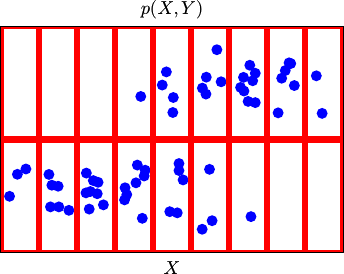
\includegraphics[width=\textwidth]{images/probability/joint.png}
        \caption{$P(X=x,Y=y)$}
        \label{fig:probability-example-joint}
    \end{subfigure}
    ~
    \begin{subfigure}[b]{0.3\textwidth}
        \centering
        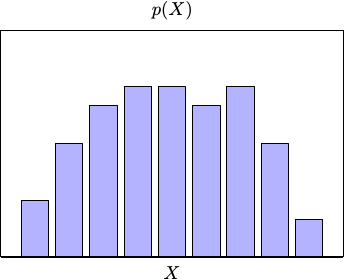
\includegraphics[width=\textwidth]{images/probability/marginal-x.png}
        \caption{$P(X=x)$}
        \label{fig:probability-example-marginal}
    \end{subfigure}
    ~
    \begin{subfigure}[b]{0.3\textwidth}
        \centering
        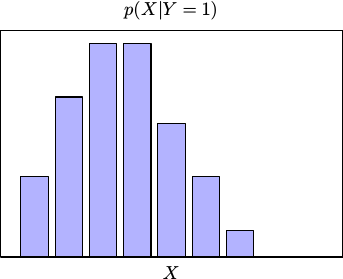
\includegraphics[width=\textwidth]{images/probability/conditional-on-y.png}
        \caption{$P(X=x|Y=1)$}
        \label{fig:probability-example-conditional}
    \end{subfigure}
    \caption[Example for joint distribution with marginal and conditional
    distribution]{Visualization of marginal (\subref{fig:probability-example-marginal}) and
        conditional (\subref{fig:probability-example-conditional}) distributions of a joint
        probability distribution (\subref{fig:probability-example-joint}) over two variables $X$ and
        $Y$ (taken and modified from \citealp[16]{bishop_07_pattern}). $X$ takes nine
        possible values, $Y$ takes two possible values ($1$ and $2$, from bottom to top). Clearly
        (\subref{fig:probability-example-marginal}) and
        (\subref{fig:probability-example-conditional}) are two different distributions and
        therefore visualize the difference between marginal and conditional distribution:
        Marginalizing over $Y$ corresponds to adding the value of each point in
        (\subref{fig:probability-example-joint}) to the corresponding bin in the histogram over $X$
        in (\subref{fig:probability-example-marginal}). The resulting distribution is not a function
        of $y$. On the contrary, conditioning $Y=1$ can be understood as selecting only that part of
        the distribution that fulfills that condition, \ie the bottom row in
        (\subref{fig:probability-example-joint}). In order to arrive at the conditional distribution
        (\subref{fig:probability-example-conditional}), the selected row needs to be normalized by
        the probability $P(Y=1)$.}
    \label{fig:probability-vis}
\end{figure}

Queries on a probability distribution for drawing conclusions are called
\emph{inference}~\citep[75]{barber_12_bayesian}. A simple query is the calculation of the
probability for a specific state of random variables. In the context of data observation, the
posterior
\begin{align}
    \label{eq:probability-posterior}
    P(\mathcal{X}|\mathcal{D}) = \frac{P(\mathcal{D}|\mathcal{X})}{P(\mathcal{D})}
\end{align}
is the distribution of random variables $\mathcal{X}$ conditioned on observations
$\mathcal{D}$~\citep[173]{barber_12_bayesian}. The mode of the posterior distribution, \ie the
variable setting
\begin{align}
    \mathcal{X}^{\text{MAP}} = \argmax_{\mathcal{X}} P(\mathcal{X}|\mathcal{D}),
\end{align}
which maximizes the posterior distribution, is called the \emph{maximum a posteriori} (MAP)
estimate. Throughout this thesis, the explicit statement of conditioning on observed data
$\mathcal{D}$ is omitted.

With the introduction of and notational conventions~(\cref{tab:probability-notation}) for random
variables and probabilities at hand, we continue with a short introduction to probabilistic
graphical models in \cref{sec:gm-graphical-models}.

% For the models presented in this thesis, the
% \emph{maximum a posteriori} (MAP) estimate~\citep[173]{barber_12_bayesian}
% \begin{align}
%     \label{eq:probability-map}
% \end{align}
% is used to infer the mode of the associated posterior probability distributions.



% A distribution $P(\mathcal{X}=\{x_1,\hdots,x_N\})=P(x_1,\hdots,x_n)$ over a set of random variables
% $\mathcal{X}=\{X_1,\hdots,X_n\}$ is called a \emph{joint distribution}. 

% \cref{def:random-var} allows for the definition of joint distributions over random variables. Due to
% the limitation to discrete random variables, all definitions refer to discrete random variables
% only. However, these definitions can be applied to conitinuous variables with only slight
% modifications (see \citet[Chapter~1]{barber_12_bayesian} and
% \citet[Chapter~2.1]{koller_09_probabilistic}). 


% Throughout this thesis we encounter only probability distributions over discrete random
% variables. Thus, without the need for an explicit declaration, all random variables are constrained
% to be discrete (including binary random variables). Furthermore, only properties of distributions over
% discrete random variables are described in the following. However, this properties hold for
% continuous random variables as well with the slight m



%%% Local Variables: 
%%% mode: latex
%%% TeX-master: "../../main"
%%% End: 
